%!TEX TS-program = xelatex
\documentclass[10pt,oneside]{article}
\usepackage[fontsize=9pt]{scrextend}

\usepackage[english]{babel}

\usepackage{amsmath,amssymb,amsfonts}
\usepackage[utf8]{inputenc}
\usepackage[T1]{fontenc}
\usepackage{stix2}
\usepackage[scaled]{helvet}
\usepackage[scaled]{inconsolata}

\usepackage{lastpage}

\usepackage{setspace}

\usepackage{ccicons}

\usepackage[hang,flushmargin]{footmisc}

\usepackage{geometry}

\setlength{\parindent}{0pt}
\setlength{\parskip}{6pt plus 2pt minus 1pt}

\usepackage{fancyhdr}
\renewcommand{\headrulewidth}{0pt}\providecommand{\tightlist}{%
  \setlength{\itemsep}{0pt}\setlength{\parskip}{0pt}}

\makeatletter
\newcounter{tableno}
\newenvironment{tablenos:no-prefix-table-caption}{
  \caption@ifcompatibility{}{
    \let\oldthetable\thetable
    \let\oldtheHtable\theHtable
    \renewcommand{\thetable}{tableno:\thetableno}
    \renewcommand{\theHtable}{tableno:\thetableno}
    \stepcounter{tableno}
    \captionsetup{labelformat=empty}
  }
}{
  \caption@ifcompatibility{}{
    \captionsetup{labelformat=default}
    \let\thetable\oldthetable
    \let\theHtable\oldtheHtable
    \addtocounter{table}{-1}
  }
}
\makeatother

\usepackage{array}
\newcommand{\PreserveBackslash}[1]{\let\temp=\\#1\let\\=\temp}
\let\PBS=\PreserveBackslash

\usepackage[breaklinks=true]{hyperref}
\hypersetup{colorlinks,%
citecolor=blue,%
filecolor=blue,%
linkcolor=blue,%
urlcolor=blue}
\usepackage{url}

\usepackage{caption}
\setcounter{secnumdepth}{0}
\usepackage{cleveref}

\usepackage{graphicx}
\makeatletter
\def\maxwidth{\ifdim\Gin@nat@width>\linewidth\linewidth
\else\Gin@nat@width\fi}
\makeatother
\let\Oldincludegraphics\includegraphics
\renewcommand{\includegraphics}[1]{\Oldincludegraphics[width=\maxwidth]{#1}}

\usepackage{longtable}
\usepackage{booktabs}

\usepackage{color}
\usepackage{fancyvrb}
\newcommand{\VerbBar}{|}
\newcommand{\VERB}{\Verb[commandchars=\\\{\}]}
\DefineVerbatimEnvironment{Highlighting}{Verbatim}{commandchars=\\\{\}}
% Add ',fontsize=\small' for more characters per line
\usepackage{framed}
\definecolor{shadecolor}{RGB}{248,248,248}
\newenvironment{Shaded}{\begin{snugshade}}{\end{snugshade}}
\newcommand{\KeywordTok}[1]{\textcolor[rgb]{0.13,0.29,0.53}{\textbf{#1}}}
\newcommand{\DataTypeTok}[1]{\textcolor[rgb]{0.13,0.29,0.53}{#1}}
\newcommand{\DecValTok}[1]{\textcolor[rgb]{0.00,0.00,0.81}{#1}}
\newcommand{\BaseNTok}[1]{\textcolor[rgb]{0.00,0.00,0.81}{#1}}
\newcommand{\FloatTok}[1]{\textcolor[rgb]{0.00,0.00,0.81}{#1}}
\newcommand{\ConstantTok}[1]{\textcolor[rgb]{0.00,0.00,0.00}{#1}}
\newcommand{\CharTok}[1]{\textcolor[rgb]{0.31,0.60,0.02}{#1}}
\newcommand{\SpecialCharTok}[1]{\textcolor[rgb]{0.00,0.00,0.00}{#1}}
\newcommand{\StringTok}[1]{\textcolor[rgb]{0.31,0.60,0.02}{#1}}
\newcommand{\VerbatimStringTok}[1]{\textcolor[rgb]{0.31,0.60,0.02}{#1}}
\newcommand{\SpecialStringTok}[1]{\textcolor[rgb]{0.31,0.60,0.02}{#1}}
\newcommand{\ImportTok}[1]{#1}
\newcommand{\CommentTok}[1]{\textcolor[rgb]{0.56,0.35,0.01}{\textit{#1}}}
\newcommand{\DocumentationTok}[1]{\textcolor[rgb]{0.56,0.35,0.01}{\textbf{\textit{#1}}}}
\newcommand{\AnnotationTok}[1]{\textcolor[rgb]{0.56,0.35,0.01}{\textbf{\textit{#1}}}}
\newcommand{\CommentVarTok}[1]{\textcolor[rgb]{0.56,0.35,0.01}{\textbf{\textit{#1}}}}
\newcommand{\OtherTok}[1]{\textcolor[rgb]{0.56,0.35,0.01}{#1}}
\newcommand{\FunctionTok}[1]{\textcolor[rgb]{0.00,0.00,0.00}{#1}}
\newcommand{\VariableTok}[1]{\textcolor[rgb]{0.00,0.00,0.00}{#1}}
\newcommand{\ControlFlowTok}[1]{\textcolor[rgb]{0.13,0.29,0.53}{\textbf{#1}}}
\newcommand{\OperatorTok}[1]{\textcolor[rgb]{0.81,0.36,0.00}{\textbf{#1}}}
\newcommand{\BuiltInTok}[1]{#1}
\newcommand{\ExtensionTok}[1]{#1}
\newcommand{\PreprocessorTok}[1]{\textcolor[rgb]{0.56,0.35,0.01}{\textit{#1}}}
\newcommand{\AttributeTok}[1]{\textcolor[rgb]{0.77,0.63,0.00}{#1}}
\newcommand{\RegionMarkerTok}[1]{#1}
\newcommand{\InformationTok}[1]{\textcolor[rgb]{0.56,0.35,0.01}{\textbf{\textit{#1}}}}
\newcommand{\WarningTok}[1]{\textcolor[rgb]{0.56,0.35,0.01}{\textbf{\textit{#1}}}}
\newcommand{\AlertTok}[1]{\textcolor[rgb]{0.94,0.16,0.16}{#1}}
\newcommand{\ErrorTok}[1]{\textcolor[rgb]{0.64,0.00,0.00}{\textbf{#1}}}
\newcommand{\NormalTok}[1]{#1}

\newlength{\cslhangindent}
\setlength{\cslhangindent}{1.5em}
\newlength{\csllabelwidth}
\setlength{\csllabelwidth}{3em}
\newenvironment{CSLReferences}[3] % #1 hanging-ident, #2 entry spacing
 {% don't indent paragraphs
  \setlength{\parindent}{0pt}
  % turn on hanging indent if param 1 is 1
  \ifodd #1 \everypar{\setlength{\hangindent}{\cslhangindent}}\ignorespaces\fi
  % set entry spacing
  \ifnum #2 > 0
  \setlength{\parskip}{#2\baselineskip}
  \fi
 }%
 {}
\usepackage{calc} % for \widthof, \maxof
\newcommand{\CSLBlock}[1]{#1\hfill\break}
\newcommand{\CSLLeftMargin}[1]{\parbox[t]{\maxof{\widthof{#1}}{\csllabelwidth}}{#1}}
\newcommand{\CSLRightInline}[1]{\parbox[t]{\linewidth}{#1}}
\newcommand{\CSLIndent}[1]{\hspace{\cslhangindent}#1}\usepackage[table,dvipsnames]{xcolor}

\geometry{includemp,
            letterpaper,
            top=2.4cm,
            bottom=2.4cm,
            left=1.0cm,
            right=1.0cm,
            marginparwidth=5cm,
            marginparsep=1.0cm}

\usepackage[singlelinecheck=off]{caption}

\captionsetup{
  font={small},
  labelfont={bf},
  format=plain,
  labelsep=quad
}

\usepackage{floatrow}

\floatsetup[figure]{margins=hangright,
              facing=no,
              capposition=beside,
              capbesideposition={center,outside},
              floatwidth=\textwidth}

% \floatsetup[table]{margins=hangright,
%              facing=no,
%              capposition=beside,
%              capbesideposition={center,outside},
%              floatwidth=\textwidth}

\pagestyle{plain}

\setcounter{secnumdepth}{5}

\usepackage{titlesec}

\titleformat{\section}[block]
{\normalfont\large\sffamily}
{\thesection}{.5em}{\titlerule\\[.8ex]\bfseries}

\titleformat{\subsection}[runin]
{\normalfont\fontseries{b}\selectfont\filright\sffamily}
{\thesubsection.}{.5em}{}

\titleformat{\subsubsection}[runin]
{\normalfont\itshape\rmfamily\bfseries}{\thesubsubsection}{1em}{}

\fancypagestyle{firstpage}
{
   \fancyhf{}
   \renewcommand{\headrulewidth}{0pt}
   \fancyfoot[R]{\footnotesize\ccby}
   \fancyfoot[L]{\footnotesize\sffamily\today}
}

\fancypagestyle{normal}
{
  \fancyhf{}
  \fancyfoot[R]{\footnotesize\sffamily\thepage\ of \pageref*{LastPage}}
}

\usepackage{tikz}
\begin{document}
\pagestyle{normal}
\thispagestyle{firstpage}

\newcommand{\colorRule}[3][black]{\textcolor[HTML]{#1}{\rule{#2}{#3}}}

\noindent {\LARGE \textbf{\textsf{Forecasting the spatio-temporal
uncoupling of bumblebee-flower interaction networks}}}

\medskip
\begin{flushleft}
{\small
%
\href{https://orcid.org/0000-0002-6506-6487}{Michael D.\,Catchen}%
%
\,\textsuperscript{1,2}, %
\href{https://orcid.org/0000-0001-9051-0597}{Francis\,Banville}%
%
\,\textsuperscript{3,4,2}, %
Paul\,CaraDonna%
%
\,\textsuperscript{5,6}, %
\href{https://orcid.org/0000-0002-2151-6693}{Dominique\,Caron}%
%
\,\textsuperscript{1,2}, %
\href{https://orcid.org/0000-0002-6248-3007}{Philippe\,Desjardins-Proulx}%
%
\,\textsuperscript{3,2}, %
\href{https://orcid.org/0000-0001-9019-0108}{Norma R.\,Forero-Muñoz}%
%
\,\textsuperscript{3,2}, %
\href{https://orcid.org/0000-0001-6075-8081}{Andrew\,Gonzalez}%
%
\,\textsuperscript{1,2}, %
\href{https://orcid.org/0000-0002-4498-7076}{Dominique\,Gravel}%
%
\,\textsuperscript{4,2}, %
Jane E.\,Ogilvie%
%
\,\textsuperscript{5}, %
\href{https://orcid.org/0000-0002-6004-4027}{Laura\,Pollock}%
%
\,\textsuperscript{1,2}, %
\href{https://orcid.org/0000-0002-0735-5184}{Timothée\,Poisot}%
%
\,\textsuperscript{3,2}, %
\href{https://orcid.org/0000-0001-6067-1349}{Tanya\,Strydom}%
%
\,\textsuperscript{3,2}, %
Julian\,Resasco%
%
\,\textsuperscript{7}
\vskip 1em
\textsuperscript{1}\,McGill University; \textsuperscript{2}\,Québec
Centre for Biodiversity Sciences; \textsuperscript{3}\,Université de
Montréal; \textsuperscript{4}\,Université de
Sherbrooke; \textsuperscript{5}\,Rocky Mountain Biological
Laboratory; \textsuperscript{6}\,Chicago Bontanic
Garden; \textsuperscript{7}\,University of Colorado Boulder\\
\vskip 1em
\textbf{Correspondance to:}\\
Michael D. Catchen --- \texttt{michael.catchen@mail.mcgill.ca}\\
}
\end{flushleft}

\vskip 2em
\makebox[0pt][l]{\colorRule[CCCCCC]{2.0\textwidth}{0.5pt}}
\vskip 2em
\noindent

\marginpar{\vskip 1em\flushright
{\small{\bfseries Keywords}:\par
species interactions\\ecological
forecasting\\pollinators\\bumbleebees\\network ecology\\}
}




        {\bfseries Purpose:}\,This template provides a series of scripts
to render a markdown document into an interactive website and a series
of PDFs.\\%
        {\bfseries Motivation:}\,It makes collaborating on text with
GitHub easier, and means that we never need to think about the
output.\\%
        {\bfseries Internals:}\,GitHub actions and a series of python
scritpts. The markdown is handled with \texttt{pandoc}.\\%
    

\vskip 2em
\makebox[0pt][l]{\colorRule[CCCCCC]{2.0\textwidth}{0.5pt}}
\vskip 2em

\emph{title ideas}: Forecasting the spatio-temporal uncoupling of
bumblebee-flower interaction networks

\hypertarget{introduction}{%
\section{Introduction}\label{introduction}}

Species interactions and climate change.

Two dimensions: spatial and temporal.

\begin{enumerate}
\def\labelenumi{\arabic{enumi})}
\tightlist
\item
  Elevation gradients.
\end{enumerate}

\begin{itemize}
\tightlist
\item
  dispersal capacity and range shifts
\end{itemize}

\begin{enumerate}
\def\labelenumi{\arabic{enumi})}
\setcounter{enumi}{1}
\tightlist
\item
  Phenological uncoupling {[}cite{]}.
\end{enumerate}

\begin{itemize}
\tightlist
\item
  Abundance is a function of time in the year
\end{itemize}

\hypertarget{methods}{%
\section{Methods}\label{methods}}

\hypertarget{data}{%
\subsection{Data}\label{data}}

\hypertarget{models}{%
\subsection{Models}\label{models}}

We denote the predicted probability of two species, \(i\) and \(j\),
interacting a \(p_{ij}\). The outcome is here is to build a model \(f\),
or rather a set of candidate models, that take \(i\) and \(j\) and
inputs, and which potentially combine this with .features

\[p_{ij} = f(i,j)\]

\hypertarget{candidate-models}{%
\subsubsection{Candidate models}\label{candidate-models}}

\textbf{\emph{True Neutral}}:
\(f(i,j) = \frac{1}{\sum_i \sum_j 1} = 1 / (P\cdot F)\)

\textbf{\emph{Relative-abundance (interaction neutral)}}:
\(f(i,j) = A_i A_j\) where \(A_x\) is the relative abundance of species
\(x\).

\textbf{\emph{Relative-abundance + environment-embedding}}:
\(f(i,j) = g(i,j, E_i, E_j)\)

\textbf{\emph{Relative-abundance + phylogeny-embedding}}: \$\$

\textbf{\emph{Relative-abundance + environment-embedding +
phylogeny-embedding}}

\begin{figure}
\hypertarget{fig:concept}{%
\centering
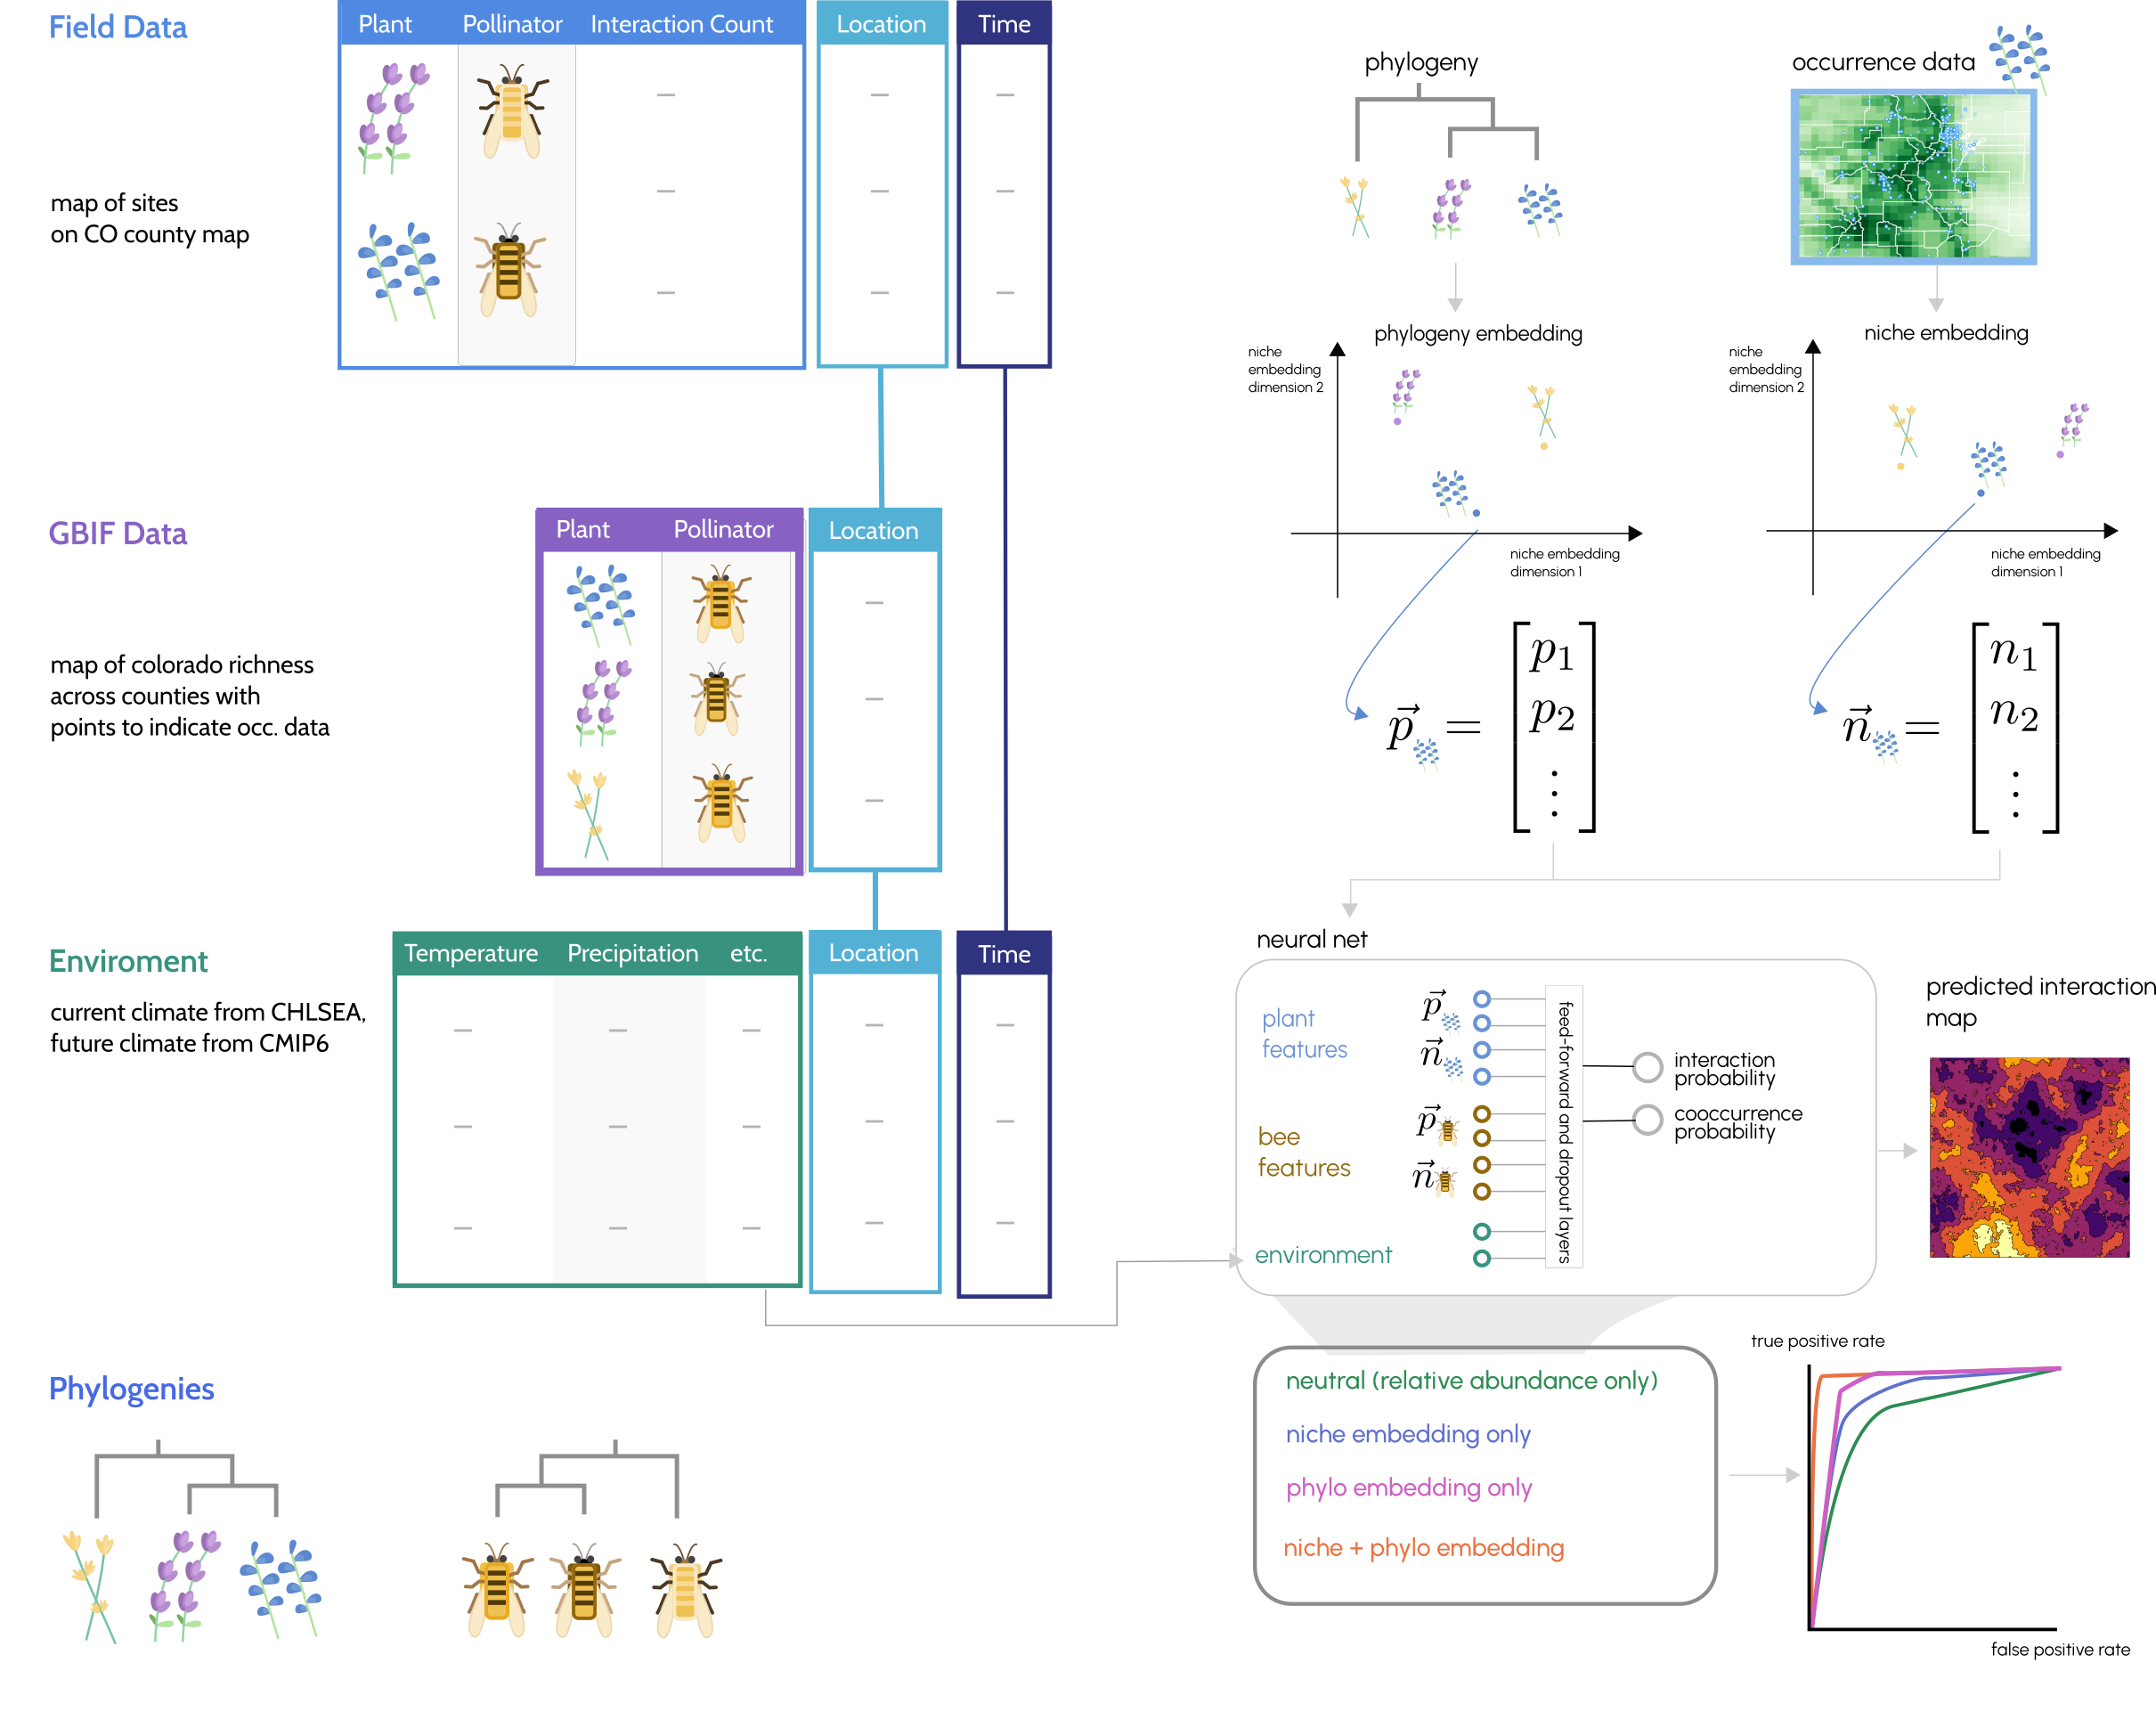
\includegraphics{./figures/concept_v2.png}
\caption{todo}\label{fig:concept}
}
\end{figure}

In gravel et al 2017
\[P(X_{iy}, X_{jy}, L_{ijy} | E_y) = P(X_{iy},X_{jy}P(L_{ijy} | X_{iy}, X_{jy}, E_y)\]
Then decompose probability of co-occurence as
\[P(X_{iy}, X_{jy}) = P(X_{iy})P(X_{jy})\]

\hypertarget{a-predictive-model-to-make-spatially-explicit-network-prediction}{%
\subsection{A predictive model to make spatially explicit network
prediction}\label{a-predictive-model-to-make-spatially-explicit-network-prediction}}

The goal is two have two predictive models: interaction-predictor model
and a distribution-predictor model (a la Strydom \& Catchen et al.~2021,
figure 2).

The interaction-predictor model, \(f_i(s_i,s_j, \theta_i)\) predicts
interaction based on species-level features \((s_i, s_j)\), and is
trained on the field-data.

These features could include Phylogeny (to be determined: how available
are genomes or trees for these species) Environment/Climate Traits (to
be determined: what trait data is available, how annoying is it to
clean) Time (only for the phenology model, see 3.2 and 3.3)

The distribution-predictor model, \(f_s(s_i, \vec{x}, t)\) is trained on
GBIF data to predict the occurrence of species with features si at a
location in space x, and time t. Many options here. Here the species
level features could be Climatic variables derived from remote sensing
products. Co-occurence to make a JSDM Potentially weighted by phenology
information from field data. Time (only for the phenology model, see 3.2
and 3.3)

\hypertarget{combining-distribution-predictor-and-interaction-predictor-models}{%
\subsection{Combining distribution-predictor and interaction-predictor
models}\label{combining-distribution-predictor-and-interaction-predictor-models}}

Can split this into two based on how the distribution-predictor works.
If \(f_s\) predicts co-occurrence, then draw the species pool first and
predict interactions between the species in that pool. If \(f_s\) is a
single-species SDM, get the occurrence probability for each species p\_s
and compute the probability of observing interaction as function of the
product of occ. prob.

\hypertarget{results}{%
\section{Results}\label{results}}

After comparing different combinations of features/model structures and
finding the `best' performing model on validation data.

\hypertarget{figure-one-spatial-species-pool-and-network-prediction}{%
\subsection{Figure one: spatial species pool and network
prediction}\label{figure-one-spatial-species-pool-and-network-prediction}}

Figure that is two panels: a map of total species richness and a map of
network properties across Colorado. This model doesn't consider time,
only other predictors.

\hypertarget{figure-two-phenology}{%
\subsection{Figure two: Phenology}\label{figure-two-phenology}}

Same as figure one but consists of maps but at different times of the
year (e.g. March, June, August) and uses both an interaction-predictor
and distribution-predictor that incorporate time into predictions

\hypertarget{figure-three-climate}{%
\subsection{Figure three: Climate}\label{figure-three-climate}}

Much as climate change has shifted temperature gradients to get warmer
toward the poles, it has also moved temperature gradients up in
elevation.

We can get a CMIP6 forecast of temperature and precipitation, and then
predict how many observed interactions in the field data will no longer
have their composing species' distributions overlap. Decompose temporal
component of overlap from spatial component.

\hypertarget{discussion}{%
\section{Discussion}\label{discussion}}

\hypertarget{acknowledgements}{%
\subsection{Acknowledgements}\label{acknowledgements}}

\hypertarget{references}{%
\section{References}\label{references}}

\end{document}
